
    % (aff 圖)
    \begin{figure}
        \centering
        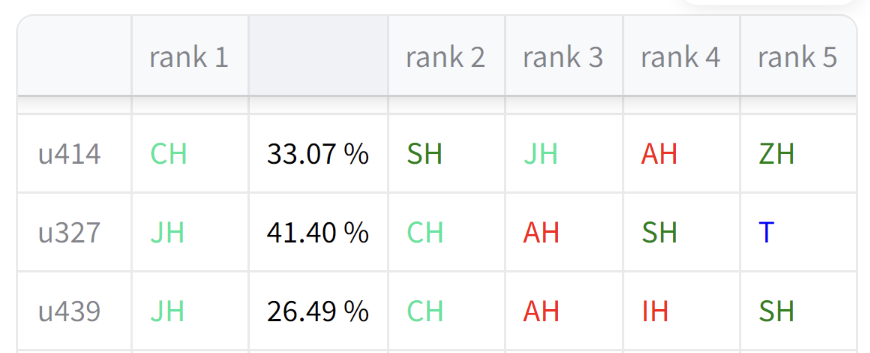
\includegraphics[width=0.8\linewidth]{figures/ch4figs/aff-hub50-500.png}
        \caption{對 HuBERT 分群數 50 離散單元取得 500 種次詞單位後,}
        對應到塞擦音的聲學片段之音位條件機率排名
        \label{fig:aff}
    \end{figure}


\begin{table}[!htbp]
    \centering
    
    \begin{subtable}[t]{\textwidth}
        \centering
        \begin{tabular}{|c|c|c|} \hline 
                符記種數& 音位分類純度& 以音位分類標註之分群純度\\ \hline 
               離散單元&   0.7006&  \textbf{0.1509}
\\ \hline 
                   500    &  0.7116&  0.0340
\\ \hline 
                  1000    &  \textbf{0.7186}&  0.0226
\\ \hline 
                  8000    &  0.7080&  0.0119
\\ \hline 
                 10000    &  0.7048&  0.0113
\\ \hline 
                 20000    &  0.6929&  0.0089\\ \hline 
        \end{tabular}
\caption{群數 = 50}
        \label{tab:ch4-new-hubert-pcls-clu050}
    \end{subtable}        

    \vfill        

    \begin{subtable}[t]{\textwidth}
        \centering
        \begin{tabular}{|c|c|c|} \hline 
                符記種數& 音位分類純度& 以音位分類標註之分群純度\\ \hline 
               離散單元&   \textbf{0.7584}&  \textbf{0.0882}\\ \hline 
                   500    &  0.7578&  0.0326
\\ \hline 
                  1000    &  0.7576&  0.0223
\\ \hline 
                  8000    &  0.7382&  0.0097
\\ \hline 
                 10000    &  0.7346&  0.0090
\\ \hline 
                 20000    &  0.7235&  0.0074
\\ \hline 
        \end{tabular}
\caption{群數 = 100}
        \label{tab:ch4-new-hubert-pcls-clu100}
    \end{subtable}    

\caption{HuBERT 模型在不同詞表大小時的語音學類別分析數據}
    \label{tab:new--hubert-pcls-results}
\end{table}
